% !TeX program = lualatex
% !TeX root = luaking.tex
% !TeX encoding = UTF-8
% !TeX spellcheck = cs_CZ
%---------------------------------------------------------------------------------------------------
% file fey1ch21.tex
%---------------------------------------------------------------------------------------------------
%=========================== Kapitola: Harmonický oscilátor ========================================
\setchaptertoc
\chapter{Harmonický oscilátor}\label{fyz:IchapXXI}
  \section{Lineární diferenciální rovnice}\label{fyz:IchapXXIsecI}
    Kurz studia fyziky se obvykle dělí na tématické části jako například mechanika, elektřina,
    optika atd., přičemž se studují jedna za druhou. Například v našem kurzu jsme se zatím většinou
    zabývali mechanikou. Znovu a znovu se však stává podivná věc: rovnice, jež se objevují v různých
    odvětvích fyziky, a dokonce i v jiných vědách, jsou často téměř stejné. Mnohé jevy mají proto
    své analogie v těchto různých odvětvích. Jako jednoduchý příklad uveďme, že šíření zvukových vln
    je v mnohém podobné šíření světelných vln. Při podrobném studiu akustiky zjistíme, že studujeme
    téměř totéž, jako kdybychom se podrobně zabývali studiem optiky. Studium nějakého jevu v jedné
    oblasti tak může rozšířit naše vědomosti v jiné oblasti. Nejlépe bude, když si od začátku
    uvědomíme, že takováto rozšíření jsou možná, neboť' jinak by možná někdo neviděl důvod, proč
    ztrácet čas a energii s něčím, co se zdá být jen malou částí mechaniky.
    
    Harmonický oscilátor, který se chystáme studovat, má blízké analogie v mnoha jiných odvětvích.
    Ať už začneme s příkladem závaží na pružině, kyvadla s malou výchylkou nebo jiných mechanických
    zařízení, studujeme ve skutečnosti určitou \textbf{diferenciální rovnici}. Tato rovnice se ve
    fyzice i v jiných vědách objevuje vždy znovu a znovu. Ve skutečnosti je částí tolika jevů, že
    její studium si zaslouží naši pozornost. Některé jevy, které popisuje tato rovnice, jsou
    oscilace tělesa na pružině, oscilace náboje v elektrickém obvodu, oscilace ladičky vytvářející
    zvukové vlny, vibrace elektronů v atomu vytvářející světelné vlny, rovnice činnosti takového
    servosystému, jakým je termostat regulující teplotu, komplikované interakce v chemických
    reakcích, růst kolonie bakterií interagujících s dodávanou potravou a otravnými látkami, které
    bakterie produkují, lišky, požírající králíky žeroucí trávu atd. Všechny tyto jevy probíhají
    podle rovnic, jež jsou si velmi podobné, a to je důvod, proč se tak podrobně zabýváme
    mechanickým oscilátorem. Tyto rovnice jsou \textbf{lineárními diferenciálními rovnicemi s
    konstantními koeficienty}. Lineární diferenciální rovnice s konstantními koeficienty je rovnice,
    která se skládá ze součtu více členů, přičemž každý člen je derivací závisle proměnné podle
    nezávisle proměnné vynásobený nějakou konstantou. Takže
    \begin{equation}\label{fyz:eq727}
      a_n\diff[n]xt +a_{n−1}\diff[n-1]xt +\cdots+a_1\diff{x}{t}+a_0x = f(t)
    \end{equation}
    se nazývá lineární diferenciální rovnicí \(n\)-tého řádu s konstantními koeficienty (každé
    \(a_i\) je konstanta).

  \section{Harmonický oscilátor}\label{fyz:IchapXXIsecII}
    Snad nejjednodušším mechanickým systémem, který se při svém pohybu řídí lineární diferenciální
    rovnicí s konstantními koeficienty, je těleso zavěšené na pružině. Pružina se nejdříve napne,
    aby vyvážila tíhu tělesa. Když nastane rovnováha, zajímáme se o vertikální výchylky tělesa z
    rovnovážné polohy (obr. 21.1). Posunutí směrem nahoru označíme \(x\) a budeme předpokládat, že
    pružina je dokonale lineární. V takovém případě síla, jíž působí pružina, když ji natáhneme, je
    přímo úměrná výchylce, tj. síla je rovna \(-kx\) (se znaménkem mínus, neboť síla působí opačným
    směrem než posunutí). Takže hmotnost tělesa krát jeho zrychlení je rovno \(-kx\)
    \begin{equation}\label{fyz:eq728}
      m\diff[2]xt = -kx
    \end{equation}
    Pro jednoduchost předpokládejme (nebo můžeme vhodně změnit jednotky času), že podíl
    \(k/m =1\). Nejdříve se budeme zabývat rovnicí
    \begin{equation}\label{fyz:eq729}
      \diff[2]xt = -x,
    \end{equation}
    ale později se vrátíme k rovnici (\ref{fyz:eq728}) s explicitně zapsanými \(k\) a \(m\).
    \begin{figure}[ht!] %\ref{fyz:fig246}
      \centering
      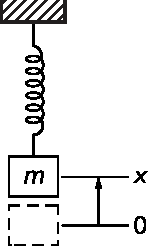
\includegraphics[width=0.3\linewidth]{fyz_fig246.pdf}
      \caption{Těleso upevněné na pružině - jednoduchý příklad harmonického oscilátoru
               (\cite[s.~287]{Feynman01})}
      \label{fyz:fig246}
    \end{figure}
    Numerickou analýzu rovnice (\ref{fyz:eq729}) jsme provedli již tehdy, kdy jsme se poprvé začali
    zabývat mechanikou. Tuto rovnici (\ref{fyz:eq129}) jsme řešili, abychom našli pohyb. Pomocí
    numerické integrace jsme dostali křivku (obr. \ref{fyz:fig102}), podle níž, bylo-li \(m\) na
    začátku vychýleno, ale jinak v klidu, se začne pohybovat směrem dolů a projde nulovou polohou.
    Dále jsme jeho pohyb nesledovali, ale samozřejmě víme, že se pohybuje směrem nahoru a dolů - že
    \emph{osciluje}. Při numerických výpočtech jsme zjistili, že rovnovážnou polohou prošla křivka v
    bodě \(t= \num{1.570}\). Délka celého cyklu je čtyřikrát větší, \(T_0 =\SI{6.28}{\s}\) „s“ (v
    našich časových jednotkách). To jsme zjistili numericky, dokud jsme ještě neznali infinitezimální
    počet. Předpokládáme, že mezi tím vás na přednáškách z matematiky seznámili s funkcí, která se
    po dvojnásobném derivování zreprodukuje se znaménkem mínus. (Samozřejmě, existují způsoby, jak
    tuto funkci najít přímo, ale ty jsou složitější, než když řešení jednoduše přijmeme.) jde o
    \(x=\cos t\). Zderivujeme-li ji, najdeme \(\diff{x}{t} = -\sin t\) a \(\diff[2]xt = -\cos t= -
    x\). Funkce \(x= \cos t\) má v bodě \(t= 0\) počáteční hodnotu \num{1} a počáteční rychlost je
    rovna nule. S takovými počátečními podmínkami jsme začínali naši numerickou analýzu. Nyní, když
    víme, že \(x= \cos t\), můžeme vypočítat přesnou hodnotu času, za který projde bodem \(x = 0\).
    Odpověď je: \(t= \frac{\pi}{2}\) nebo \num{1.57108}. V důsledku chyb při numerické analýze jsme
    se zmýlili v poslední číslici, ale byla to velmi blízká hodnota!

    Abychom se dostali dále při řešení problémů, vrátíme se s jednotkami času ke skutečným sekundám.
    Jaké je potom řešení? Na začátku se můžeme domnívat, že konstanty \(k\) a \(m\) se nám podaří
    zahrnout, jestliže \(\cos t\) něčím vynásobíme. Zkusme tedy \(x=A\cos t\). Potom \(\diff{x}{t}=
    -A\sin t\) a \(\diff[2]xt = -A\cos t= - x\).

    K našemu překvapení vidíme, že jsme neuspěli v řešení rovnice (\ref{fyz:eq728}), ale znovu jsme
    dostali rovnici (\ref{fyz:eq729})! Tato skutečnost je ilustrací jedné z nejdůležitějších
    vlastností lineárních rovnic: \emph{Vynásobíme-li nějaké řešení libovolnou konstantou, dostaneme
    znovu řešení téže rovnice.} Matematický důvod je jasný. Je-li \(x\) řešením a vynásobíme-li obě
    strany rovnice \(A\), pak všechny derivace jsou vynásobeny \(A\), a proto \(Ax\) je právě tak
    dobré řešení, jako bylo \(x\). Fyzikální důvod je takový: Stáhneme-li závaží zavěšené na pružině
    dolů dvakrát tak daleko než dříve, síla je dvojnásobná, výsledné zrychlení je dvojnásobné,
    rychlost získaná za danou dobu je dvojnásobná a vzdálenost prošlá za danou dobu je dvojnásobná.
    Ale těleso \emph{musí} projít dvojnásobnou vzdálenost, aby se dostalo zpět do počátku, protože
    jsme ho na začátku vychýlili dvakrát tak daleko. Takže do počátku se vrátí za stejnou dobu, bez
    ohledu na velikost počáteční výchylky. Jinými slovy: Pohyb popsaný lineární rovnicí má stejný
    \emph{časový průběh} bez ohledu na to, jak velkou silou byl vyvolán.

    Neprovedli jsme správnou úpravu – jen jsme se poučili, že řešení můžeme vynásobit jakoukoli
    konstantou a bude vyhovovat stejné rovnici, avšak ne jiné rovnici. Po takovýchto pokusech s
    násobením \(x\) nějakou konstantou zjišťujeme, že musíme změnit časově měřítko. Jinak řečeno,
    rovnice (\ref{fyz:eq728}) má řešení ve tvaru
    \begin{equation}\label{fyz:eq730}
      x=\cosω_0t.
    \end{equation}
    (Je důležité si uvědomit, že v tomto případě \(\omega_0\) není úhlovou rychlostí rotujícího
    tělesa, ale kdybychom nesměli použít stejné písmeno k označení více než jedné věci, neměli
    bychom dost písmen.) Důvod, proč jsme označili \(\omega\) indexem nula je ten, že za chvíli
    budeme mít více symbolů \(\omega\). Zapamatujme si, že \(\omega_0\) odpovídá přirozenému pohybu
    oscilátoru. Nyní zkusme dosadit do rovnice (\ref{fyz:eq730}). Jsme na tom lépe, neboť
    \(\diff{x}{t}=−ω_0\sinω_0t\) a
    \begin{equation*}
      \diff[2]xt = −ω^2_0\cosω_0t = −ω^2_0x
    \end{equation*}
    Takže na konec jsme přece jen vyřešili rovnici, kterou jsme chtěli řešit. Rovnice \(\diff[2]xt =
    −ω^2_0x\) je stejná jako rovnice (\ref{fyz:eq727}), jestliže \(\omega_0^2 = k/m\).

    Dále musíme prozkoumat fyzikální význam \(ω_0\). Víme, že funkce kosinus se opakuje s periodou
    \(2\pi\). Takže \( x=\cosω_0t\) bude opakovat stejný pohyb (projde celým cyklem), změní-li se
    „úhel“ o \(2\pi\). Veličina \(ω0t\) se často nazývá \textbf{fází pohybu}. Abychom změnili
    \(ω0t\) o \(2π\), musí se čas změnit o hodnotu \(T_0\), která se nazývá periodou jedné úplné
    oscilace. Samozřejmě musí platit, že \(\omega_0T_0 = 2\pi\), tj. \(\omega_0T_0\) musí odpovídat
    jednomu cyklu úhlové proměnné a všechno se zopakuje, zvětšíme-li \(t\) o \(T_0\) a fázi o
    \(2\pi\). Takže
    \begin{equation}\label{fyz:eq731}
      t_0=\frac{2π}{ω_0}=2π\sqrt{\frac{m}{k}}
    \end{equation}  
    Budeme-li mít těžší závaží, budou oscilace pružiny trvat déle. Je to proto, že závaží má větší
    setrvačnou hmotnost a protože síly jsou stejné, potrvá déle, než se závaží rozhýbe. Bude-li
    pružina silnější, bude pohyb rychlejší, a to souhlasí: Je-li pružina silnější, perioda se
    zkracuje.

    Všimněme si, že perioda kmitu závaží na pružině nezávisí na tom, jak pohyb začal, jak daleko
    pružinu vychýlíme. \emph{Perioda} oscilací je určena rovnicí pohybu (\ref{fyz:eq728}), ale není
    jí určena amplituda. Taje určena tím, jak pohyb začneme, tím čemu říkáme \emph{počáteční
    podmínky}.

    Ve skutečnosti jsme ještě nenašli nejobecnější možné řešení rovnice (\ref{fyz:eq727}). Existují
    i jiná řešení. Je jasné proč - všechny případy popsané \(x = a \cos\omega_0 t\) začínají s
    počátečním posunutím a nulovou počáteční rychlostí. Ale pohyb například může začít, když je
    \(x=0\) a tělesu dodáme úderem rychlost v čase \(t= 0\). Takový pohyb není popsán kosinem, ale
    sinem. Jinak lze problém formulovat i takto: Je-li \(x = \cos\omega_0 t\) řešením, pak není
    zřejmé, zda bude pohyb stejný i tehdy, kdy náhodou vejdeme do místnosti v nějakém okamžiku
    (který nazveme „\(t= 0\)“) a uvidíme těleso jak právě prochází polohou \(x= 0\). Proto \(x =
    \cos\omega_0 t\) nemůže být nejobecnějším řešením, musí být možné posunout začátek času. Jako
    příklad můžeme řešení napsat takto: \(x = a \cos\omega_0(t - t_1)\), kde \(t_1\) je nějaká
    konstanta. To odpovídá posunutí začátku času do nějakého jiného okamžiku. Dále můžeme psát
    \begin{equation*}
      \cos(ω_0t+Δ) = \cosω_0t\cosΔ−\sinω_0t\sinΔ,
    \end{equation*}
    a
    \begin{equation*}
      x = A\cosω_0t+B\sinω_0t,
    \end{equation*}
    kde \(A=a\cosΔ\) a \(B=−a\sinΔ\). Libovolný z těchto tvarů lze použít k zápisu obecného řešení
    rovnice (\ref{fyz:eq727}), tj. každé řešení diferenciální rovnice \(\diff[2]xt=−ω^2_0x\), které
    existuje, lze napsat jako
    \begin{subequations}\label{fyz:eq732}
      \begin{align}
        x=a\cosω_0(t−t_1),        \label{fyz:eq732a}\\
        x=a\cos(ω_0t+Δ),          \label{fyz:eq732b}\\
        x=A\cosω_0t+B\sinω_0t.    \label{fyz:eq732c}
      \end{align}
    \end{subequations}
    

  \section{Harmonický pohyb a pohyb po kružnici}\label{fyz:IchapXXIsecIII}
    \begin{figure}[ht!] %\ref{fyz:fig247}
      \centering
      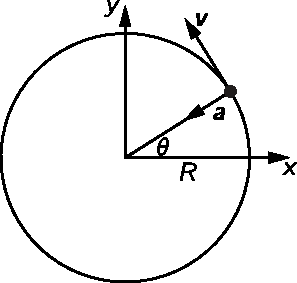
\includegraphics[width=0.5\linewidth]{fyz_fig247.pdf}
      \caption{Částice pohybující se po kruhové dráze konstantní rychlostí
              (\cite[s.~290]{Feynman01})}
      \label{fyz:fig247}
    \end{figure}

    \begin{figure}[ht!] %\ref{fyz:fig248}
      \centering
      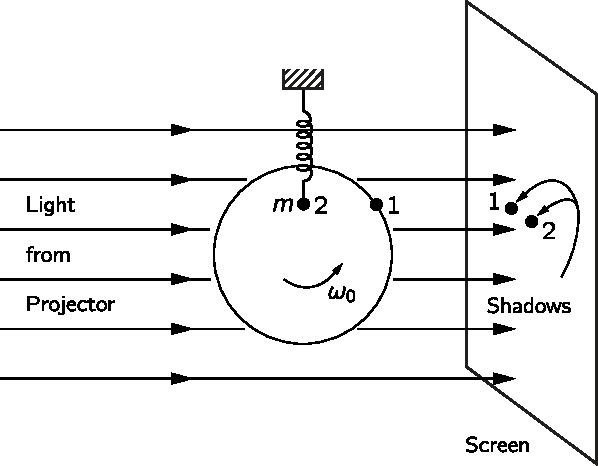
\includegraphics[width=0.5\linewidth]{fyz_fig248.pdf}
      \caption{Demonstrace ekvivalence jednoduchého harmonického pohybu a rovnoměrného pohybu po 
              krunici
              (\cite[s.~290]{Feynman01})}
      \label{fyz:fig248}
    \end{figure}

  \section{Počáteční podmínky}\label{fyz:IchapXXIsecIV}
  \section{Nucené kmity}\label{fyz:IchapXXIsecV}
  \section{Příklady a cvičení}\label{fyz:IchapXXIsecVI}

%---------------------------------------------------------------------------------------------------